\hypertarget{cmd:seite-einrichten}{}
\hypertarget{cmd:druck-vorschau}{}
\hypertarget{cmd:drucken}{}
\hypertarget{cmd:drucken-alles}{}
\hypertarget{cmd:drucker-einrichten}{}
\section{Drucken / Plotten}
\label{sec:print_plot}
Bevor Sie die Zeichnung zum Drucker bzw. Plotter schicken, haben Sie noch weitere
M�glichkeiten, die Seite einzurichten.
Innerhalb einer Arbeitssitzung mit \wspplot\ k�nnen Sie eine Standard Seiten-
/Druckereinrichtung �ber \menu{Datei / Druckereinrichtung (Standard) } festlegen (Abb. \ref{fig:seite-einrichten}).
Hier w�hlen Sie den zu verwendenden Drucker sowie die Papiergr��e aus und legen die
R�nder (Abstand Papierrand-Rahmen) fest. Nachdem Sie die Standarddruckereinrichtung
festgelegt haben, werden alle Profile, die Sie danach �ffnen, automatisch mit dieser
Standarddruckereinrichtung formatiert. Genau die gleichen Einstellungen lassen sich unter
\menu{Datei / Seite einrichten} f�r einen Einzelplot festlegen. Die Standardeinstellungen
bleiben nur so lange g�ltig, wie das Programm nicht wieder geschlossen wird.

\begin{figure}[hbtp]
	\begin{center}
		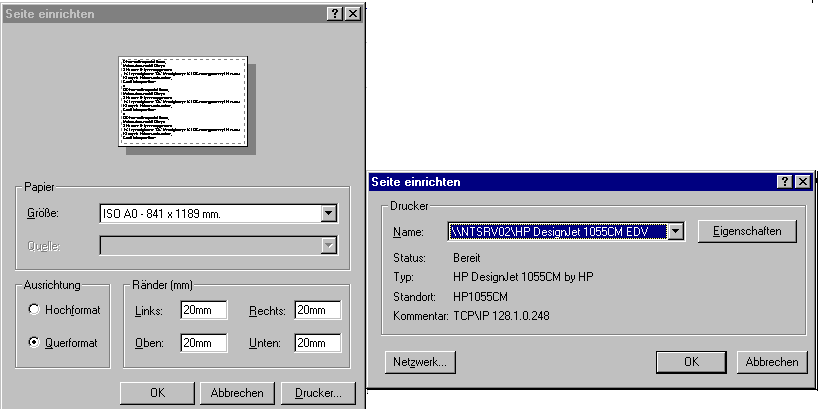
\includegraphics[scale=0.70]{seite-einrichten}
	\end{center}
	\caption{Seite einrichten}
	\label{fig:seite-einrichten}
\end{figure}

�ber \menu{Datei / Drucken} schicken Sie den Plot zu ihrem Ausgabeger�t.
